\chapter{Implementation}
\label{chap:dpp}

\section{Data Pre-processing}
In this section, we discuss various attempts made to reduce the search space and unnecessary recursion calls to save time and space. Following techniques have been used:

\subsection{Candidate List Generation}

\begin{frame}{}
\begin{algorithm}
\caption{\textsc{getCandidates}}\label{euclid}

\textbf{Input:} Data graph g, Query graph q, Data vertex v.\\
\textbf{Output:} Candidate set of all $u \in V(q)$

\begin{algorithmic}[1]
\State $Candidate \gets \emptyset$\\
\Comment{\textcolor{green}{For all $v \in V(g)$, we launch a thread. Each thread performs the following operation}}

\ForAll{$u \in V(q)$}
\If{$degree(v) > degree(u)$ \&\& $L(u) = L(v)$}
    \State \textcolor{blue}{index = atomicIncrement(numCandidates(u))}
    \State \textcolor{blue}{$Candidate(u, index) \gets v$}
\EndIf
\EndFor
\State \textbf{return} $Candidate$
\end{algorithmic}
\end{algorithm}
\end{frame}

This process helps to reduce the search space by identifying those vertices of data graph which can possibly be a match for any vertex of query graph. For a particular vertex u of a query graph, A vertex v of data graph is said to be a candidate iff:
\begin{itemize}
    \item $|v| \geq |u|$
    \item $L(v)=L(u)$
\end{itemize}

\begin{figure}[h!]
\begin{center}
        \centering
        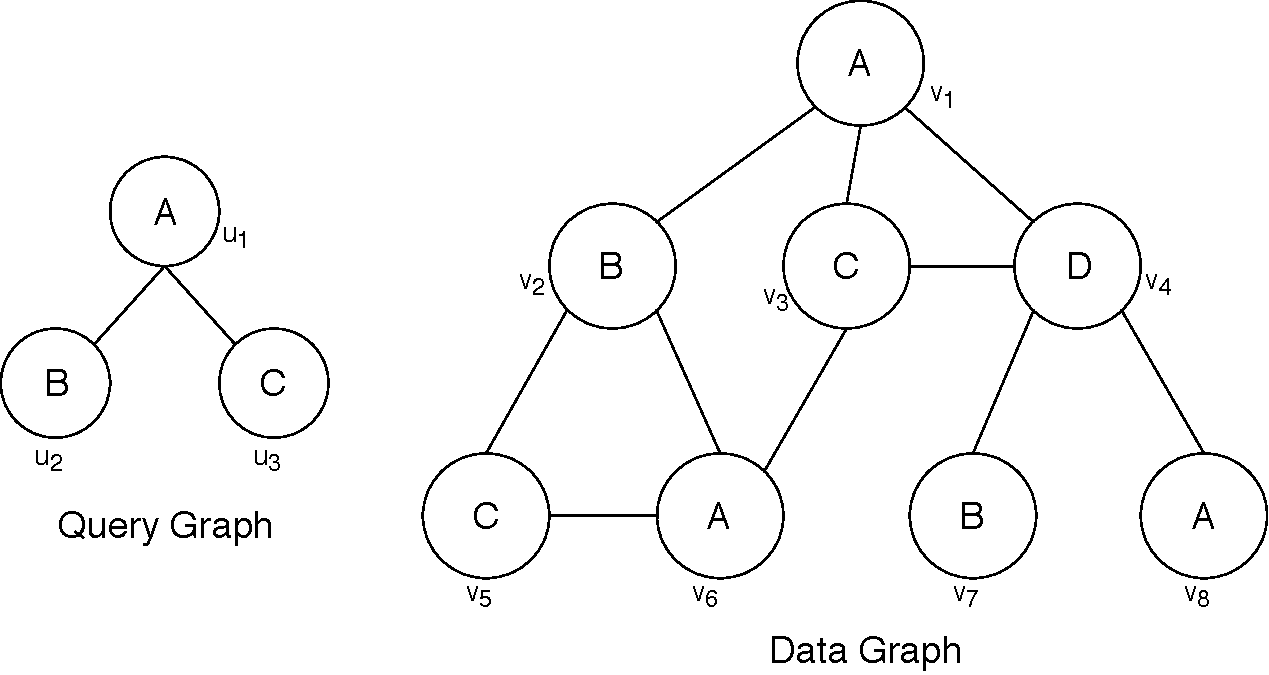
\includegraphics[width=\textwidth]{images/Implementation.pdf}
        \caption{Data Graph g and Query Graph q}
        \label{fig:flowchart}
\end{center}
\end{figure}

Consider the data graph and query graph as shown. As per the definition, the candidate list of $u_1$ = \{$v_1, v_6$\}, candidate list of $u_2$ = \{$v_2, v_7$\} and $u_3$ = \{$v_3, v_5$\}.

In the parallel implementation of the method, we launch a thread for every vertex v of data graph. Each thread then finds all the query vertices of which v can be a candidate of. Since there is a data race between each thread to add a vertex $v \in V(d)$ to the candidate set of vertex $u \in V(q)$, atomicInc is used to prevent any data hazard due to the race. The numCandidate(u) returns the number of candidates of a vertex $u \in V(q)$ found so far.

\section{Query vertex ordering}

The order in which \textsc{FindMatch} processes the query vertex also determines the time of execution of algorithm. In order to have an efficient query vertex ordering, we suggest the following score function given to each query vertex:
\[
score(u) = N(L(u), g)/|v|
\]
where N(L(u), g) is the number of vertices in the data graph with the same label as that of u. The query vertices are then sorted in ascending order of their score. For e.g. for the graphs in figure 3.1, the order of query vertices will be $u_1$-$u_2$-$u_3$ with scores of 1.5, 2 and 2. The idea behind this scoring function is that higher the degree of a node, the more likely it is to get pruned while searching for a match. Inversely, the lesser the number of vertices in data graph with the same label as that of u, the more likely it will get pruned faster. However this may not always be the best choice.

\section{Algorithm}

In the parallel implementation of the Algorithm, first, we obtain all the candidate set of vertices of the query graph. Then we obtain the order in which we are to process the query vertices. These processes have been discussed in the previous section.

In the parallel implementation of \textsc{findMatch}, we select the first query vertex that is to be processed. For each candidate of the query vertex, we launch a thread that calls \textsc{subgraphSearch}. The \textsc{subgraphSearch} procedure recursively checks for the candidates of the next query vertex that is to processed. If the candidate is joinable, i.e. the corresponding edges between the vertices in M and the corresponding vertices in q exist, then candidate is added to M.

For example, in the graph shown in figure 3.2, vertex $u_1$ is selected and two threads are launched which search for the match from vertices $v_6$ and vertex $v_1$ respectively. The threads then check for the candidates of vertices to follow. Say $thread\_0$  is launched corresponding to the vertex $v_1$, it will check for the candidates of the vertex $u_2$. Since the corresponding edges between the vertices \{$u_1$, $u_2$\} and \{$v_1$, $v_2$\} exist,  vertex $v_2$ is added to M and the state is updated. Similarly, since the corresponding edges between the vertices \{$u_1$, $u_2$\} and \{$v_1$, $v_7$\} do not exist, the vertex $v_7$ is discarded. Next, candidates of vertex $u_3$ are checked. In the graph, since the vertices \{$u_1$, $u_2$, $u_3$\} and \{$v_1$, $v_2$, $v_3$\} have the corresponding edges matched, the procedure \textsc{SubgraphSearch} reports it as a match. Since corresponding edges between \{$u_1$, $u_2$, $u_3$\} and \{$v_1$, $v_2$, $v_5$\} do not match, $v_5$ is discarded and the function returns.

\begin{figure}[]
\begin{center}
        \centering
        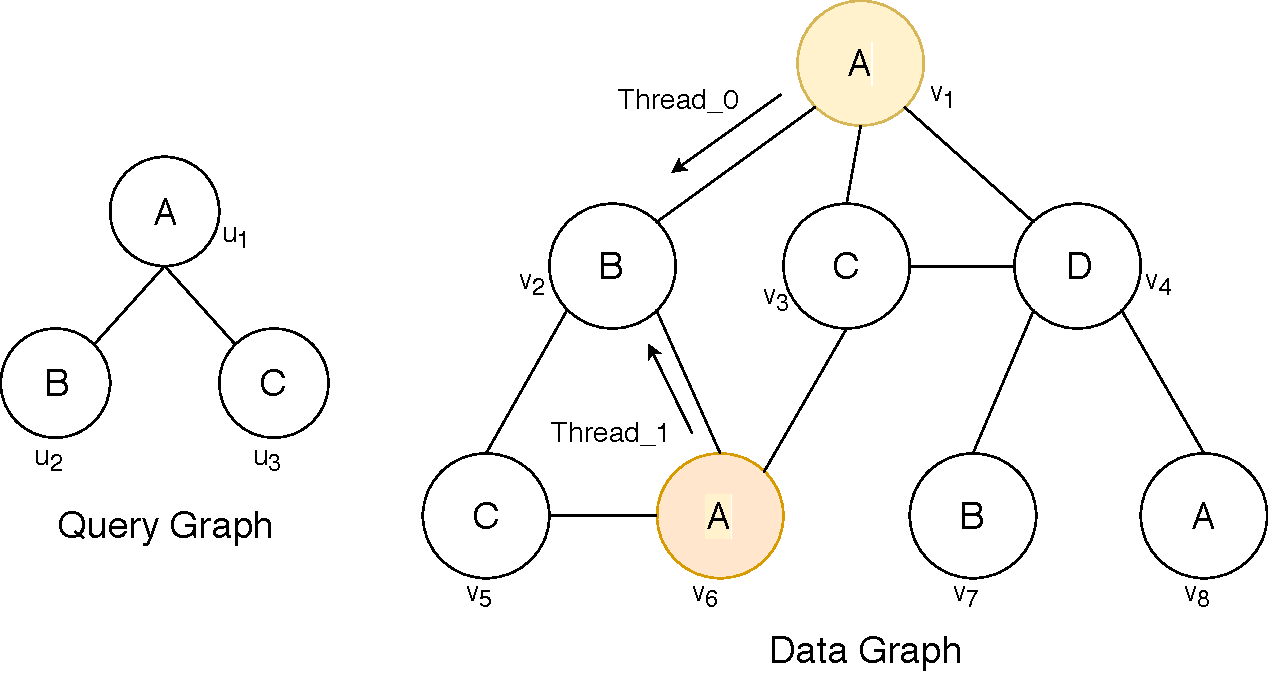
\includegraphics[width=\textwidth]{images/Implementation_thread.pdf}
        \caption{\textsc{SubgraphSearch}}
        \label{fig:flowchart}
\end{center}
\end{figure}

Similarly, say $thread_1$ is launched corresponding to the vertex $v_6$. Similar procedure is performed i.e. vertex $v_2$ is added to M. In the next recursive call, both vertices $v_3$ and $v_5$ report a match. While the vertex $v_7$ is discarded because the corresponding edges do not match. Hence the the algorithm reports the match \{$v_1$, $v_2$, $v_3$\} (reported by thread\_0), \{$v_6$, $v_2$, $v_5$\} and \{$v_6$, $v_2$, $v_3$\} (reported by thread\_1).

\begin{frame}{}
    \begin{algorithm}
\caption{\textsc{FindMatch}}\label{euclid}
\textbf{Input:} Data graph g, Query graph q, Candidate set C, Order of processing Query vertices\\
\textbf{Output:} all subgraph isomorphisms of q in g.

\begin{algorithmic}[1]
\State $M \gets \emptyset$
\State $C \gets \textsc{getCandidates}$
\State $u \gets \textsc{NextQueryVertex}$
\State \textsc{UpdateState(M, u, v...)}\\
\Comment{\textcolor{green}{For each $u' \in C(u)$, we launch a thread. each of which performs following operation}}
\State $\textsc{SubgraphSearch}(u^{'}, q, g, M,...)$ 
\Procedure{$\textsc{SubgraphSearch}(u, q, g, M,...)$}{}[0]
\If{$|M| = |V(q)|$}
    \State \textsc{\textcolor{blue}{lock()}}
    \State \textbf{report} M
    \State \textsc{\textcolor{blue}{unlock()}}
    \Else
    \State $u^{'} \gets \textsc{NextQueryVertex}$
    
    \ForAll{$v \in C(u^{'})$}
        
        \If{\textsc{$\sim$ IsVisited(v)}}
    
            \If{\textsc{IsJoinable}(q, g, M, u, v)}
                    \State \textsc{UpdateState(M, u, v...)}
                    \State $\textsc{SubgraphSearch}(u, q, g, M,...)$
            \Else
                    \State RestoreState(M, q, g, )
                    \State \textbf{return}
            \EndIf
        \EndIf

    \EndFor
    
\EndIf
\EndProcedure{}
\end{algorithmic}
\end{algorithm}
\end{frame}


\section{Challenges}

\subsection{Recursive Implementation}

Initially, the algorithm was implemented using recursion. However, since CUDA supports recursive implementation upto 24 levels, the algorithm did not work for query graph of size 8 vertices. To overcome this problem, the recursive procedure is implemented by maintaining stack. Following pseudocode shows stack implementation of \textsc{SubgraphSearch}


\begin{frame}{}
    \begin{algorithm}
\caption{\textsc{SubgraphSearch\_Stack}}\label{euclid}
% \textbf{Input:} Data graph g, Query graph q, Candidate set C, Order of processing Query vertices\\
% \textbf{Output:} all subgraph isomorphisms of q in g.
\begin{algorithmic}[1]
\State $M \gets \emptyset$
\State $C \gets \textsc{getCandidates}$
\State $u \gets \textsc{NextQueryVertex}$
\State \textsc{push} $u$
\While{$\sim$ \textsc{stackEmpty}}
    \State \textsc{pop}
    
    \If{$|M| = |V(q)|$}
        \State \textsc{\textcolor{blue}{lock()}}
        \State \textbf{report} M
        \State \textsc{\textcolor{blue}{unlock()}}
        
    \Else
        \If{\textsc{$\sim$ IsVisited(v)}}
            \If{\textsc{IsJoinable}(q, g, M, u, v)}
                \State \textsc{UpdateState(M, u, v...)}
                \State \textsc{push} next candidate of current query vertex
                \State \textsc{push} a candidate of next query vertex
            \EndIf
            
        \Else
            \State \textsc{push} $u$
        \EndIf
    \EndIf
\EndWhile

\end{algorithmic}
\end{algorithm}
\end{frame}




\subsection{Exponential Complexity}

Because of the exponential complexity of the algorithm, a number of implementational challenges were faced. One of them being the use of dynamic parallelism. Since at each step number of calls increase exponentially, so does the number of threads. Hence dynamic parallelism is not used for implementing the algorithm.
